% File name: Reports/Second Report/Andy_Second_Int_Report.tex
% Second Interim Report for GF2 Software project.
% Includes code listings/alterations and description, test definition
% files and circuit diagrams and a single page user guide.
% Author: adh
% Date: Fri May 31 00:52:24 BST 2013

\documentclass[a4paper,10pt]{article}  % Standard document class
\usepackage[english]{babel}            % Set document language
\usepackage{fullpage}                  % Set up page for small margins etc

\usepackage{graphicx}                  % For including images in document
\usepackage{placeins}                  % Allows use of \FloatBarrier
% to avoid images or tables
% moving into next section
\usepackage{subfig}                    % For subfigures...

\usepackage{amsmath}                   % For improving maths/formula typesetting
%\usepackage{tabularx}                  % Table changing package

%\usepackage{algpseudocode}             % For producing algorithms/flowcharts

\usepackage{color}
\definecolor{grey}{rgb}{0.5,0.5,0.5}

\usepackage{listings}                  % For including source code in document
\lstset{
  basicstyle = \footnotesize\ttfamily,
  commentstyle = \color{grey},
  keepspaces = true,
  keywordstyle = \color{blue},
  language = C++,
  numbers = left,
  numbersep=5pt,
  numberstyle=\tiny\color{grey},
  stepnumber=5,
  tabsize=2,
}

% Provide command for scientific notation
\providecommand{\e}[1]{\ensuremath{\times10^{#1}}}
\providecommand{\degrees}{\ensuremath{^{\circ}}}

% Define title here:
\title{Project GF2: Software\\ Second Interim Report\\ Software Design
  Team 1}
\author{George Ayris\\ gdwa2\\ Emmanuel \\ Parser \& Scanner \and James Glanville\\
jg597\\ Emmanuel \\ Scanner \& Parser \and \textbf{Andrew Holt}\\
\textbf{ah635}\\ \textbf{Emmanuel}\\ \textbf{GUI}}
\date{31 May 2013}

\begin{document}

% generate title
\maketitle

\section{Introduction}
\label{sec:introduction}

This report gives a brief summary of the graphical user interface
(gui) development for the GF2 Software Project. Version 1.0 of the
logic simulation package has been produced and tested. In addition to
the program file listings, test files for the software and the
corresponding circuit diagrams are shown. Finally, a single page user
guide describing the operation of the software package is given.

\section{File Listings and Descriptions}
\label{sec:file-list-descr}

For the gui development, the vast majority of my code has been in the
\texttt{gui.h} and \texttt{gui.cc} files, and primarily concerned with
the \texttt{MyFrame} class, with some fairly minor modifications made
to the \texttt{MyGLCanvas} class. These files are listed in full in
appendix 

The header file, \texttt{gui.h}, contains the class and function
templates for \texttt{MyFrame} and \texttt{MyGLCanvas}. It also
contains an \texttt{enum} type, defining the widgets used in the gui.

The main file, \texttt{gui.cc}, contains the definitions for
\texttt{MyFrame} and \texttt{MyGLCanvas}. Considerable modifications
have been made to the \texttt{MyGLCanvas::Render} method. For the gui
implemented, multiple canvases were required, each showing just a
single trace. For this purpose, an \texttt{int} was passed to the
function to determine which monitor to use to get the trace. The
contents of the \texttt{MyGLCanvas::OnMouse} was deleted as no mouse
interaction is desired. The code will be completely removed given more
time to ensure no adverse side effects are brought about by the
removal of the function.

The event table is defined starting from line 126. This ties the
events generated by the user interaction to the functions and
procedures defined in the callback functions.

The constructor underwent heavy modification to produce a more
flexible, more usable user interface. The canvases are stored in a
vector, and two more vectors contain the sizers and labels for the
canvases. This design offers great flexibility and easy control over
multiple traces, and they can be easily hidden and shown to avoid
unnecessary traces distracting from the important information.

Additionally, a terminal style text output was implemented in the gui
to display error messages. A particular challenge was to ensure that a
monospaced font was used in the text display so that the error
messages are displayed correctly and showing the error in the right
place.

The callback functions are largely self explanatory. One neat feature
in these is the implementation of the \texttt{OnAddMonitor} and
\texttt{OnRemMonitor}, which ensure that the multiple canvases and
sizers display correctly and the lists of monitors that may be added
or removed are properly maintained.

\section{Test Files and Circuit Diagrams}
\label{sec:test-files-circuit}

Two main test files were used to test the whole system. In addition to
these, many test files with carefully devised errors were used for
testing the parser and scanner. A limited amount of user testing was
run to 1ensure the gui operated as expected.

The first test file defines a four bit shift register. This type of
circuit uses bistables to pass signals through the array on each clock
pulse (by convention, they tend to be rising edge triggered). Shift
registers find heavy application in driving serial buses from parallel
data sources, among many other applications. The circuit diagram is
shown in figure . The definition file is listed in appendix
\ref{sec:definition-files}.
\begin{figure}[htb]
  \begin{center}
    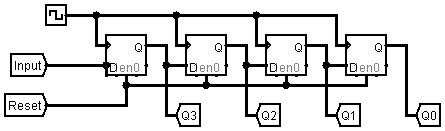
\includegraphics[width=0.8\textwidth]{shift.png}
  \end{center}
  \caption{4 bit shift register.}
  \label{fig:shiftreg}
\end{figure}

The other main testing file defined a simple gate array. The gate
array was selected as it utilises all of the required gate
types. Between the gate array and the shift register all the devices
required are tested. While this particular gate array has no specific
purpose, logic gate arrays are very common in digital electronic
design, and the design of such circuits would be a primary usage of a
software package such as this. The circuit diagram is shown in figure
\ref{fig:loggates}. The definition file is shown in appendix
\ref{sec:definition-files}.
\begin{figure}[htb]
  \begin{center}
    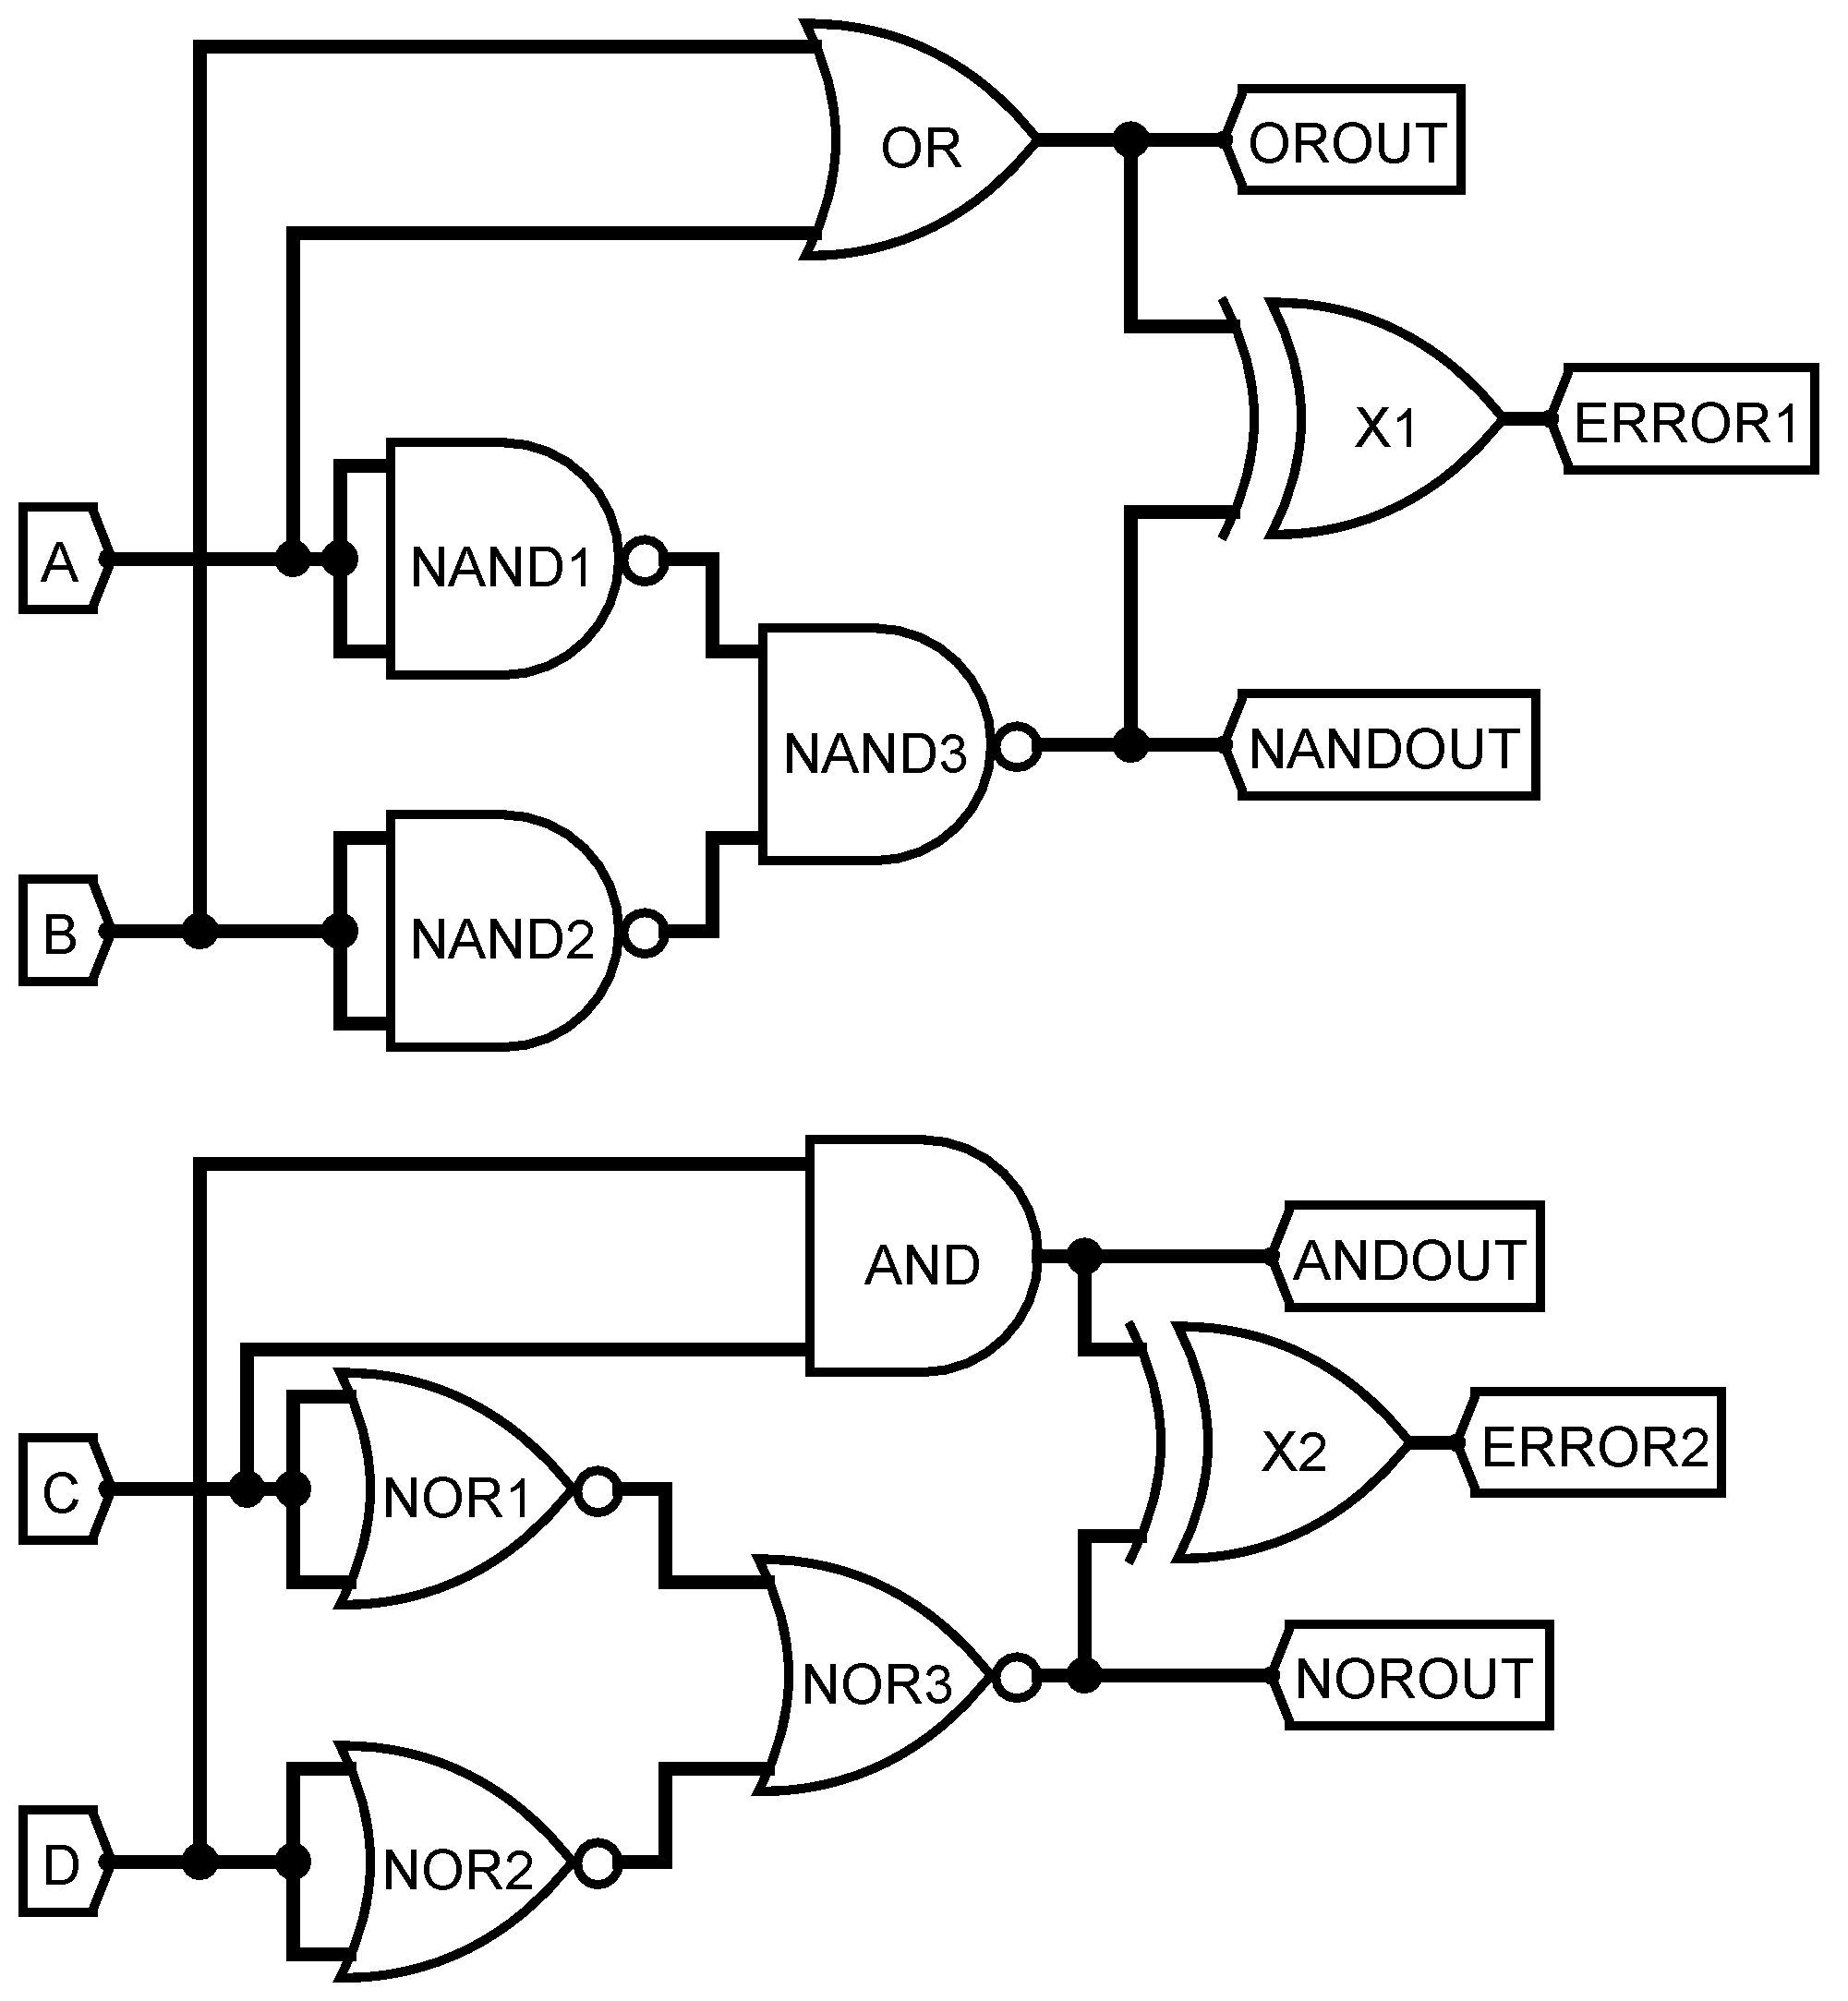
\includegraphics[width=0.6\textwidth]{testgates.png}
  \end{center}
  \caption{Logic Gate Array}
  \label{fig:loggates}
\end{figure}

\section{User Guide}
\label{sec:user-guide}

\subsection{Starting the Program}

The logic simulation package may be run by running the command
\texttt{./logsim} in the directory of the compiled file. The definition file to
be tested should be passed as an argument.\footnote{Development of a
  file selection dialogue from within the main graphical interface has
  begun, but was not polished or tested enough to make it into this
  release.} 

\subsection{Definition Errors}

Any errors in the definition file will be highlighted in the message
display at the bottom of the program window. This will give detailed
information about the cause and location of the error, making
debugging fast and efficient. Once all errors have been corrected the
program may be run fully.

\subsection{Setting up Monitors and Switches}

Once the definition file has been loaded, the \textbf{load} button
should be pressed. This loads the monitors and switches into the
dropdown menus for selection. To add a monitor point, simply select
the desired monitor from the list in the \textbf{add monitor}
drop-down menu. They may be removed by selecting from the
\textbf{remove monitor} menu. To ensure all required information is
visible together, without many distracting and irrelevant output
traces, up to 10 monitors may be observed at once. The value of a
switch may be set at any time during the simulation by selecting the
desired switch from the \textbf{switches} drop-down menu, followed by
the level to be set from the \textbf{switch value} menu.

\subsection{Running and Continuing the Simulation}

To run the simulation, simply select the number of clock cycles to
simulate in a single run (between 1 and 50), then press the run
button. The traces for all defined monitors will be shown. The
simulation may be continued, to observe the long term behaviour or to
investigate the effect of a changed switch level on the circuit. The
simulation may be run for up to 350 clock cycles. If the simulation is
run for a large number of cycles, the traces may no longer be
visible. In this case, simply drag the window to become wider and the
traces will increase in size so that more clock cycles are visible. 

\begin{figure}[htb]
  \begin{center}
    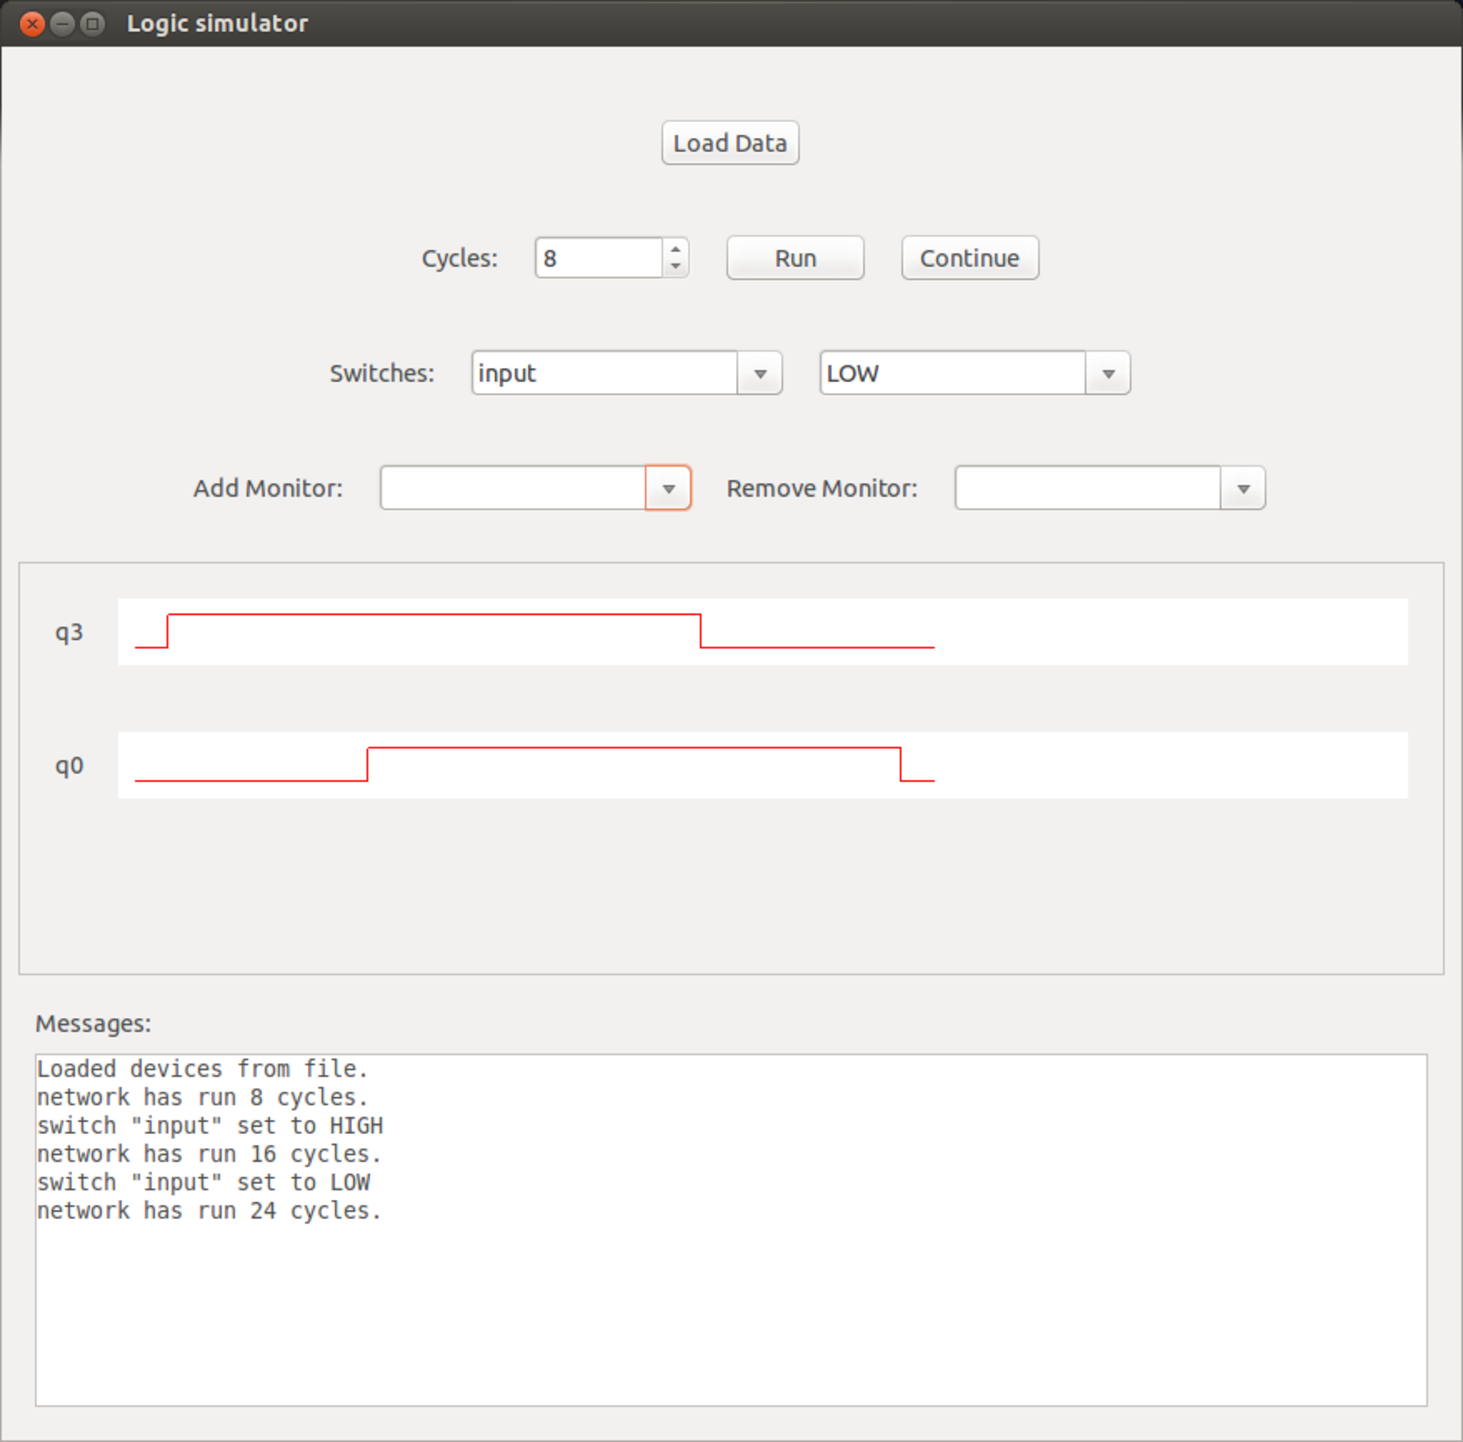
\includegraphics[width=0.8\textwidth]{Screenshot.pdf}
  \end{center}
  \caption{Screenshot of Logic Simulator Running.}
  \label{fig:scrnsht}
\end{figure}

\newpage
\appendix

\section{Source Code}
\label{sec:source-code}

\subsection{gui.h}
\label{sec:gui.h}

\lstinputlisting{gui.h}

\subsection{gui.cc}
\label{sec:gui.cc}

\lstinputlisting{gui.cc}

\section{Definition Files}
\label{sec:definition-files}

\subsection{4 Bit Shift Register}
\lstinputlisting[language=VHDL,keywordstyle=\color{black}]{shift_register.def}

\subsection{Logic Gate Array}
\lstinputlisting[language=VHDL,keywordstyle=\color{black}]{testgates.def}


\end{document}